\documentclass[usenames,dvipsnames]{beamer}
% \linespread{1.3}
\mode<presentation>{
\usetheme{Madrid}
\usecolortheme{default}
%\usecolortheme{beaver}
}
\usepackage{array}
\usepackage[utf8]{inputenc}
\usepackage{utopia}
\usepackage{verbatim}
\usepackage[portuguese]{babel}
\usepackage{pgfplots}
\pgfplotsset{/pgf/number format/use comma,compat=newest}
\usepackage{color}
\usepackage{amsmath,amsfonts,amssymb}
\usepackage{hyperref}
\usepackage{tikz}
\usepackage{caption}
\usepackage{soul}
%https://www.overleaf.com/project/61717826e515873b24296576
\usepackage{graphicx}
\usepackage{algorithm2e}
\usepackage{algorithmic}
\usepackage{xcolor}
% \usepackage{setspace}

\usetikzlibrary{positioning}

\setlength{\parskip}{1em}

\newcommand\ldiaarg[1]{\langle#1\rangle}

\newcommand{\M}{\mathcal{M}}
\newcommand{\LL}{\mathcal{L}} %for automata

\newcommand{\POL}{\mathsf{POL}}
\newcommand{\EPL}{\mathsf{EPL}}
\newcommand{\Decide}{\mathsf{Decide}}
\newcommand{\DecidePSPACE}{\mathsf{mcPOL}}
\newcommand{\reach}{\mathsf{PSPACEReach}}
\newcommand{\CreateDelta}{\mathsf{CreateDelta}}
\newcommand{\StringRepresent}{\mathsf{StringRepresent}}
\newcommand{\StoreStrings}{\mathsf{StoreStrings}}
\newcommand{\ResidueByLetter}{\mathsf{ResidueByLetter}}
\newcommand{\ResidueByWord}{\mathsf{ResidueByWord}}
\newcommand{\AuxOut}{\mathsf{AuxOut}}
\newcommand{\GetSetNP}{\mathsf{GetSetNP}}
\newcommand{\T}{\mathsf{True}}
\newcommand{\Fa}{\mathsf{False}}
\newcommand{\tr}{\mathsf{tr}}
\newcommand{\starfree}{\mathsf{Star\mbox{-}Free}}
\newcommand{\word}{\mathsf{Word}}
\newcommand{\existential}{\mathsf{Existential}}
\newcommand{\PSPACE}{\mathsf{PSPACE}}
\newcommand{\NPSPACE}{\mathsf{NPSPACE}}
\newcommand{\PTime}{\mathsf{P}}
\newcommand{\NP}{\mathsf{NP}}
\newcommand{\PTIME}{\mathsf{PTIME}}
\newcommand{\automaton}{\mathcal A}
\newcommand{\modelM}{\mathcal M}
\newcommand{\languageof}[1]{L({#1})}
\newcommand{\set}[1]{\{#1\}}
\newcommand{\suchthat}{\mid}
\newcommand{\union}{\cup}
\newcommand{\Union}{\bigcup}
\newcommand{\ep}{\ensuremath{\varepsilon}}

\newcommand{\obsright}{\blacktriangleright}
\newcommand{\obsleft}{\blacktriangleleft}
\newcommand{\obsup}{\blacktriangle}
\newcommand{\obsdown}{\blacktriangledown}

\newcommand{\expwater}{(\obsright \union \obsup)^* (\obsdown \union \obsleft \union \ep) (\obsright \union \obsup)^*}
\newcommand{\exppower}{(\obsleft \union \obsdown)^* (\obsup \union \obsright \union \ep) (\obsleft \union \obsdown)^*}
\newcommand{\exppatrol}{(\obsright^+ \obsdown^+ \obsleft^+ \obsup^+)^*}

\newcommand\drone{
\includegraphics[height=3ex]{images/E1D2_color.png}}
\newcommand\agentA{
\includegraphics[height=3ex]{images/agent A icon.png}}
\newcommand\agentB{
\includegraphics[height=3ex]{images/agent b icon.png}}
\newcommand\water{
\includegraphics[height=3ex]{images/1F4A7_color.png}}

\newcommand\algoaccept{\textbf{accept}}
\newcommand\algoreject{\textbf{reject}}

\renewcommand{\phi}{\varphi}

\tikzstyle{rectNode} = [rectangle, text centered]
\tikzstyle{fastate} = [circle, text centered, draw = black]
\tikzstyle{dots} = [circle, draw = black, fill = black, inner sep=1pt]

\tikzstyle{world} = [draw]
\tikzstyle{worldwhite} = [draw = white]

\makeatletter
\let\HL\hl
\renewcommand\hl{%
  \let\set@color\beamerorig@set@color
  \let\reset@color\beamerorig@reset@color
  \HL}
\makeatother



\title[]{Complexity Study of Reasoning about Knowledge and Public Observations}
\author[]{
\textbf{Avijeet Ghosh}\inst{1}}
\institute[Indian Statistical Institute, Kolkata]{\inst{1} Indian Statistical Institute, Kolkata\\~\\
Joint work with\\
Sourav Chakraborty, Sujata Ghosh, Fran{\c{c}}ois Schwarzentruber}
\date[September 2023]

\AtBeginSection[]
{
\begin{frame}{Table of Contents}
\tableofcontents[currentsection]
\end{frame}
}


\begin{document}

\begin{frame}
 \maketitle
\end{frame}
\begin{frame}{Table of Contents}
    \tableofcontents
\end{frame}

\section{Background}
\begin{frame}{How to Model Real-Life Scenarios}
    How do we mathematically model certain scenarios?\pause
    \begin{itemize}
        \setlength\itemsep{1em}
        \item<2-> Graphs, Flows, Linear Programs

        \item<3-> \textbf{Problem}: Static. Does not adapt to change!
        \begin{itemize}
            \setlength\itemsep{1em}
            \item<4-> \textcolor{red}{Propositional Language (Valuation models)}: In a scenario where certain facts are true, whether another fact holds true?

            \item <5-> \textcolor{red}{First-Order Language (Domain-Interpretation models)}: Is there an element in $\mathbb{N}$ which is less than every other element in it?

            \item <6-> \textcolor{red}{Context-Free Language}: Is a certain program correct syntactically?

            \item <7-> \textcolor{red}{Timed Automata}: Does an automated program written for railway gates keep the gates closed even AFTER the train leaves?

            \item <8-> \textcolor{red}{Buchi Automata}: Is an OS arriving at a deadlock EVENTUALLY?
        \end{itemize}
    \end{itemize}
\end{frame}

\newcommand{\txtimg}[3]{\raisebox{#1}{\includegraphics[scale = #2]{#3}}}

\begin{frame}{Modelling Knowledge}
    \begin{itemize}
    \setlength\itemsep{1em}
        \item<1-> How about modelling \textbf{Knowledge}?

        \item<2-> 3 people ($A, B, C$) picks one card each from a deck of 3 cards ($1, 2, 3$).

        \item<3-> How to consider \textbf{KNOWLEDGE OF AGENTS}?
        \begin{itemize}
        \setlength\itemsep{1em}
            \item<4-> \textbf{Considering possibilities}: Say $B -> $\textcolor{green}{$2$}, $B$ knows: \txtimg{-2.5mm}{0.1}{images/card-possibleBoC1.png} OR \raisebox{-2.5mm}{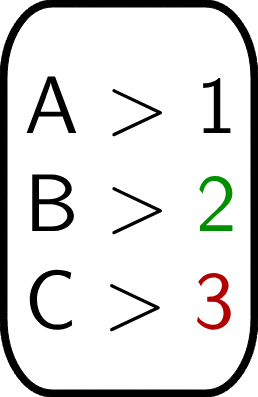
\includegraphics[scale= 0.1]{images/card-possibleBoC3.png}}

            \item<5-> \textbf{Depends on agents}: Unlike $B$, for $A$: \txtimg{-2.5mm}{0.1}{images/card-possibleA1oB2.png} OR \txtimg{-2.5mm}{0.1}{images/card-possibleA1oB3.png} 

            \item<6-> \textbf{Event changes Knowledge}: $A$ tells $B$ it has $1$, now for $B$: \txtimg{-2.5mm}{0.1}{images/card-possibleBoC3.png}
        \end{itemize}

        \item<7-> Epistemic Logic, Dynamic Epistemic Logic, Epistemic Temporal Logic
    \end{itemize}
\end{frame}

\begin{frame}{Model Checking vs Satisfiability}     ``  
    We ask these questions:\pause
    \begin{itemize}
    \setlength\itemsep{1em}
        \item<2-> Two kind of questions using Linear Programs:
        \begin{itemize}
        \setlength\itemsep{1em}
            \item<3-> Given \textbf{values of the variables} in a \textbf{Linear Programming instance}, is it a feasible solution of the instance?

            \item<4-> Given a \textbf{Linear Program instance}, does it have a feasible solution?
        \end{itemize}

        \item<5-> Two Questions involving OS programs:
        \begin{itemize}
        \setlength\itemsep{1em}
            \item<6-> Given \textbf{an OS source code}, would it eventually arrive at deadlock?

            \item<7-> Given my \textbf{specifications}, such as "the program should never arrive at a deadlock", etc, can the required program be synthesised?
        \end{itemize}
    \end{itemize}
\end{frame}


\begin{frame}{Motivation:A Farming Drone}
    \begin{figure}
        \centering
        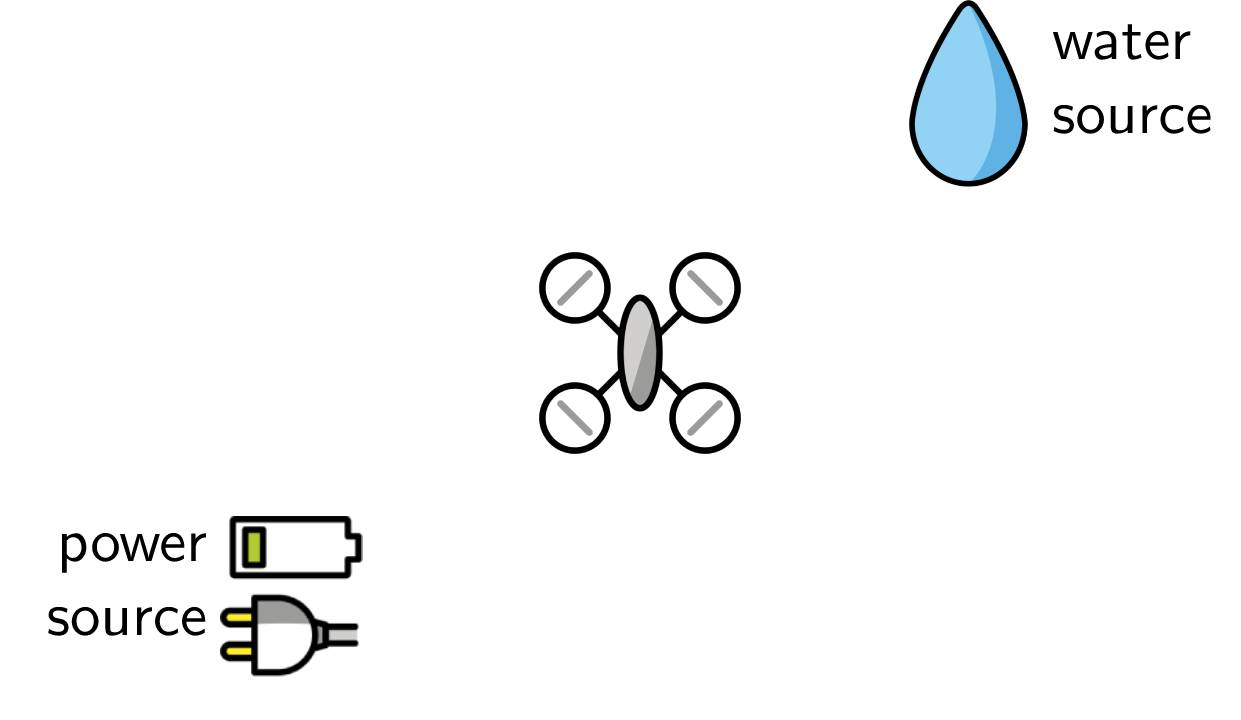
\includegraphics[scale=0.15]{images/drone-water-power.jpg}
    \end{figure}
    \begin{itemize}
        \item A water source on top right corner
        \item A power source on bottom right corner
    \end{itemize}
\end{frame}

% \begin{frame}{A Farming Drone}
%     \begin{figure}
%         \centering
%         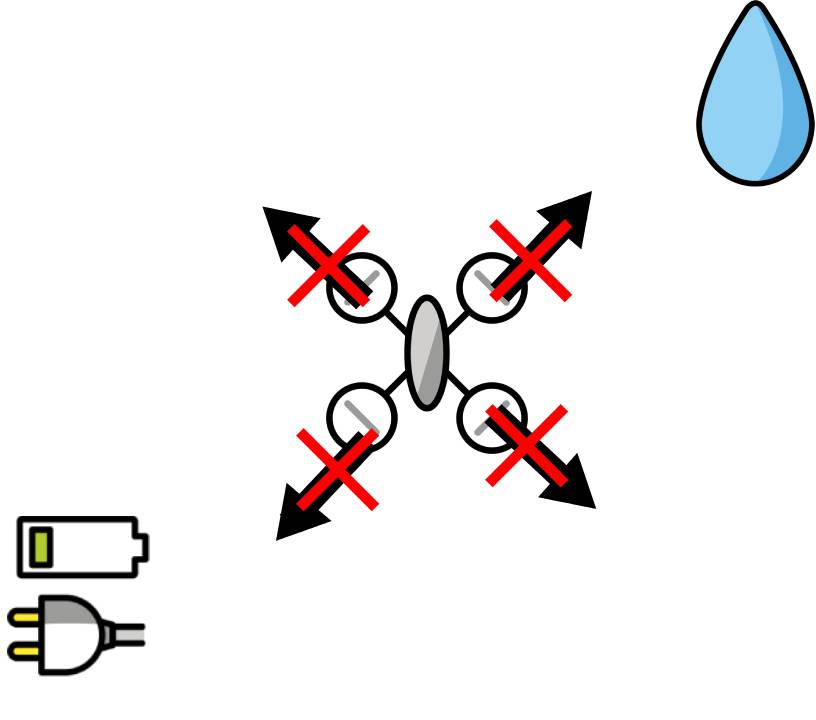
\includegraphics[scale=0.15]{images/no-diag.jpg}
%     \end{figure}
%     \begin{itemize}
%         \item Cannot move diagonally
%     \end{itemize}
% \end{frame}

\begin{frame}{Motivation:A Farming Drone}
    \begin{figure}
        \centering
        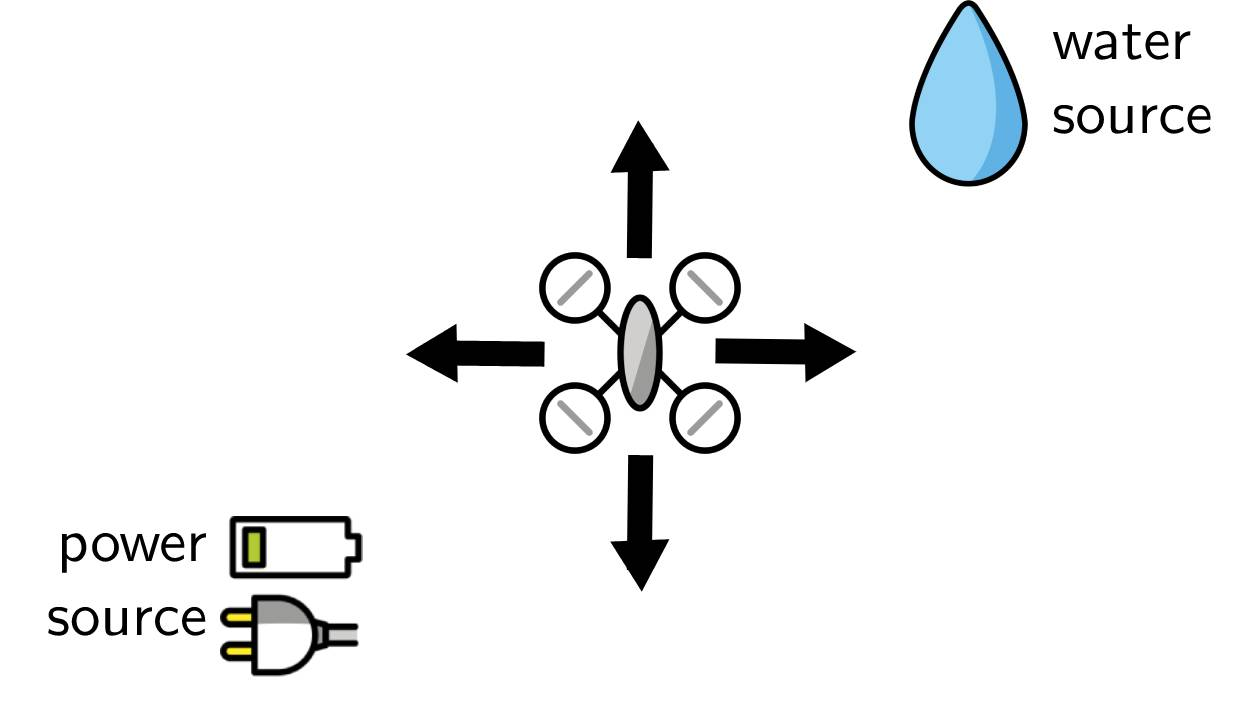
\includegraphics[scale=0.15]{images/drone-move.jpg}
    \end{figure}
    \begin{itemize}
        \item Can move up, down, left or right
        \item Cannot move diagonally
    \end{itemize}
\end{frame}

% \begin{frame}{Farming Drone: Agents}
%     \begin{figure}
%         \centering
%         
\includegraphics[scale=0.2]{images/a-expects.jpg}
%         
\includegraphics[scale=0.2]{images/b-expects.jpg}
%     \end{figure}
%     \begin{itemize}
%         \item Two agents: A and B
%     \end{itemize}
% \end{frame}

% \begin{frame}{Farming Drone: Agents}
%     \begin{figure}
%         \centering
%         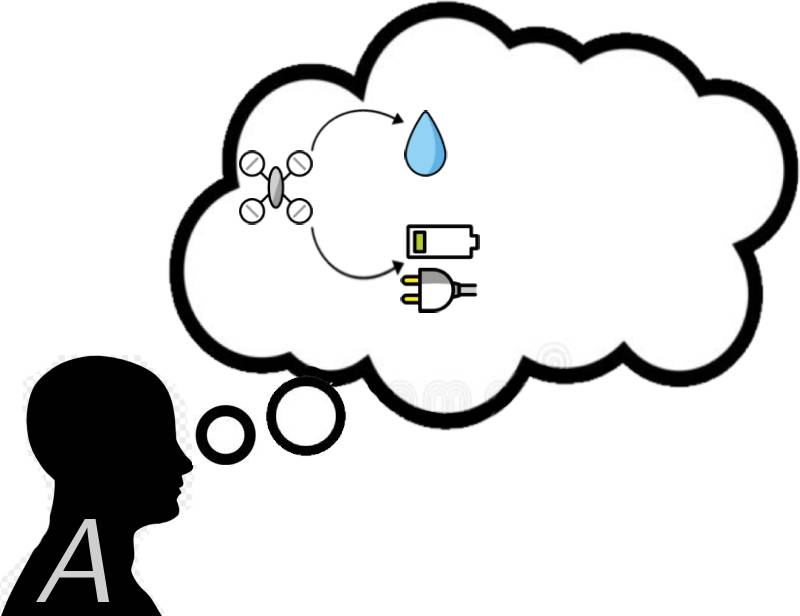
\includegraphics[scale=0.2]{images/a-expects-move.jpg}
%         
\includegraphics[scale=0.2]{images/b-expects.jpg}
%     \end{figure}
%     A expects
%     \begin{itemize}
%         \item Drone moves towards water or power source with at most one error move.
%     \end{itemize}
% \end{frame}

\begin{frame}{Farming Drone: Agents and their expectations}
    \begin{figure}
        \centering
        
\includegraphics[scale=0.2]{images/a-expects.jpg}
        
\includegraphics[scale=0.2]{images/b-expects.jpg}
    \end{figure}
     \begin{columns} 
% Column 1
    \begin{column}{.5\textwidth}
    \begin{itemize}
        \item[\textcolor{white}{\textbullet}] \textcolor{white}{Go to water with $\leq 1$ wrong move.}
        \item[\textcolor{white}{\textbullet}] \textcolor{white}{Go to power with $\leq 1$ wrong move.}
        \item[\textcolor{white}{\textbullet}] \textcolor{white}{Go patrolling in clockwise direction.}
    \end{itemize}
    \end{column}
% Column 2    
    \begin{column}{.5\textwidth}
        
    \end{column}
    \end{columns}
\end{frame}


\begin{frame}{Farming Drone: Agents and their expectations}
    \begin{figure}
        \centering
        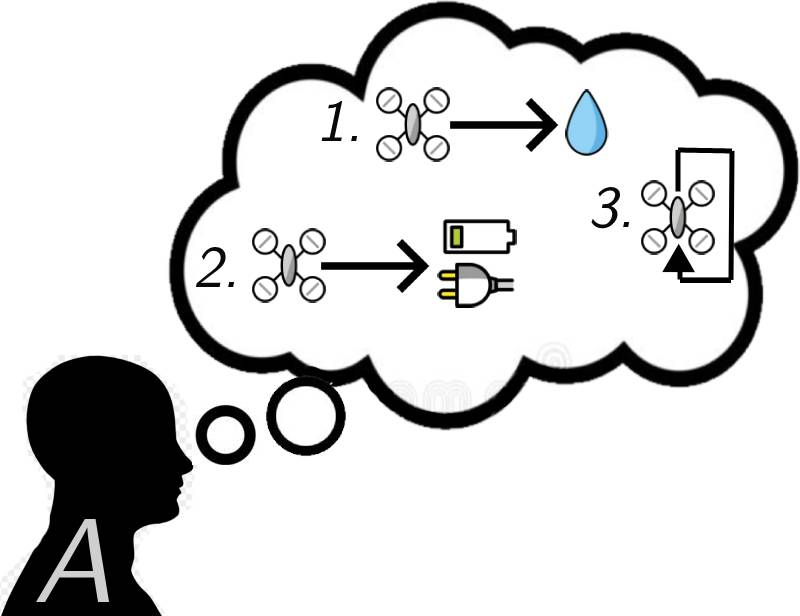
\includegraphics[scale=0.2]{images/a-expects-patrol.jpg}
        
\includegraphics[scale=0.2]{images/b-expects.jpg}
    \end{figure}
     \begin{columns} 
% Column 1
    \begin{column}{.5\textwidth}
    \begin{enumerate}
        \item Go to water with $\leq 1$ wrong move.
        \item Go to power with $\leq 1$ wrong move.
        \item Go patrolling in clockwise direction.
    \end{enumerate}
    \end{column}
% Column 2    
    \begin{column}{.5\textwidth}
        
    \end{column}
    \end{columns}
\end{frame}

\begin{frame}{Farming Drone: Agents and their expectations}
    \begin{figure}
        \centering
        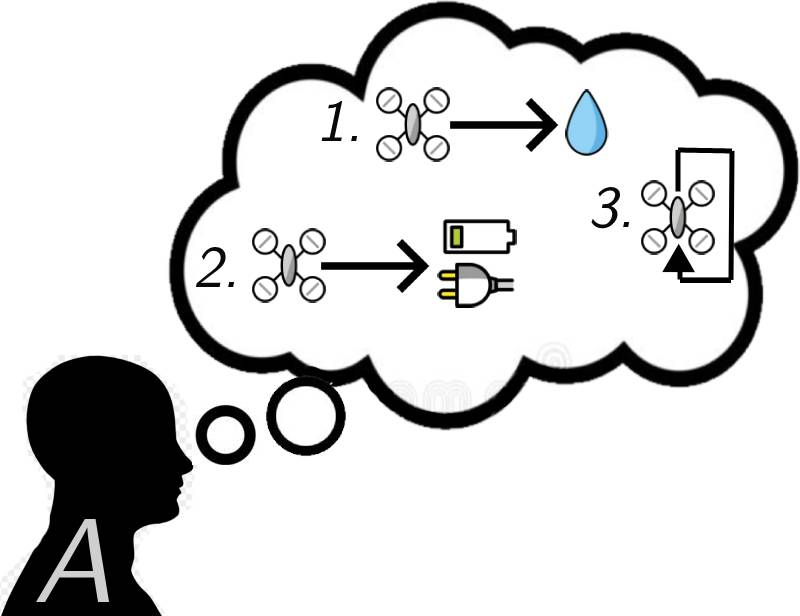
\includegraphics[scale=0.2]{images/a-expects-patrol.jpg}
        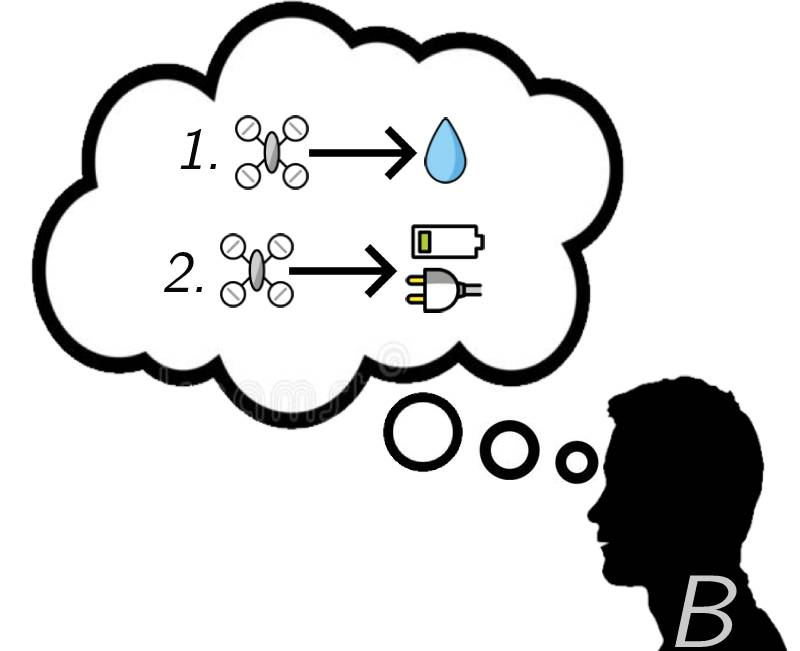
\includegraphics[scale=0.2]{images/b-expects-move.jpg}
    \end{figure}
    \begin{columns} 
% Column 1
    \begin{column}{.5\textwidth}
    \begin{enumerate}
        \item Go to water with $\leq 1$ wrong move.
        \item Go to power with $\leq 1$ wrong move.
        \item Go patrolling in clockwise direction.
    \end{enumerate}
    \end{column}
% Column 2    
    \begin{column}{.5\textwidth}
    \begin{enumerate}
        \item Go to water with $\leq 1$ wrong move.
        \item Go to power with $\leq 1$ wrong move.
    \end{enumerate}
    \end{column}
    \end{columns}
\end{frame}

\begin{frame}{Farming Drone: Reasoning about this scenario}
    \begin{columns}
    \begin{column}{0.3\textwidth}
    \begin{figure}
        \centering
        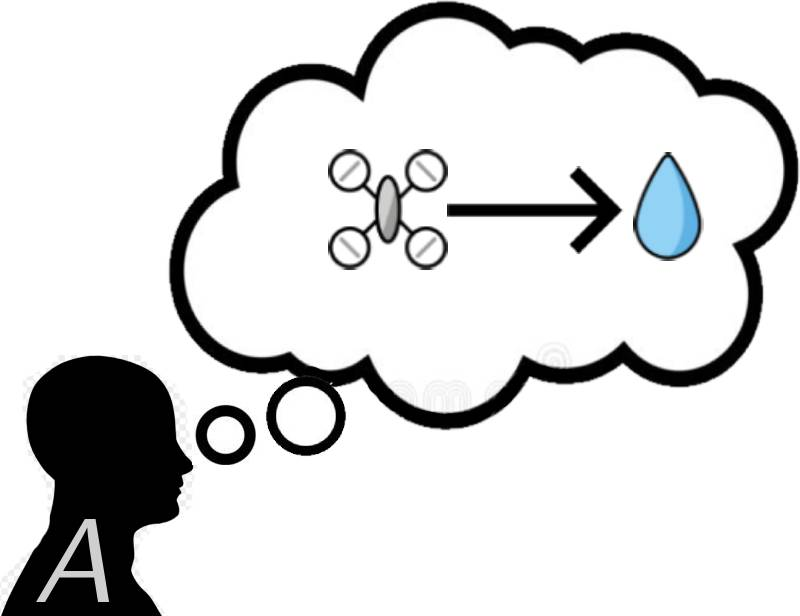
\includegraphics[scale=0.15]{images/farming A-towardsWater.jpg}
    \end{figure}
    \end{column}
    \begin{column}{0.7\textwidth}
    \begin{itemize}
        \item<1-> What is the minimal number of \raisebox{-1.5mm}{\drone} moves that A has to \textbf{observe} to know its goal?
        \item<2-> Does there exist a sequence of \raisebox{-1.5mm}{\drone} moves such that by observing it, B would know its goal but A would not?
    \end{itemize}
    \end{column}
    \end{columns}
    
\end{frame}

\begin{frame}{Modelling Knowledge: Epistemic Model}
    \begin{itemize}
         \item Epistemic model (W, R, V).
        \item[\textcolor{white}{\textbullet}] \textcolor{white}{Each world is assigned with a regular expression: a set of expected observations.}
        % \item[\textcolor{white}{\textbullet}] \textcolor{white}{Each expression is expected observations in that particular possible world.}
        \item[\textcolor{white}{\textbullet}] \textcolor{white}{Model can get truncated after an observation, say $\obsright\obsdown\obsleft$.}
    \end{itemize}
    \begin{figure}
%         \begin{tikzpicture}
% 			\node at (8, 1.5) {$W = \{u, s, t\}$};
% 			\node at (8, 1) {$V: u\leftarrow patrol, s\leftarrow water, t\leftarrow power$};
% 			\node at (8, 0.5) {$R : (u-A-s), (u-A-t), (s-A-t), (s-B-t)$};
% 		\end{tikzpicture}\\
        \pause
        \begin{tikzpicture}[yscale=1.3]
			\node[world] (s) {$water$};
			\node at (-0.5, -0.4) {\textcolor{white}{\small$\expwater$}};
			\node[world] (t) at (4, 0) {$power$};
			\node at (4.5, -0.4) {\textcolor{white}{\small$\exppower$}};
			\node[world] (u) at (0, 1) {$patrol$};
			\node at (2.3, 1) {\textcolor{white}{\small$\exppatrol$}};
			\node[left = 0mm of s] {$s$};
			\node[right = 0mm of t] {$t$};
			\node[left = 0mm of u] {$u$};
			\draw (s) edge node[above] {$A,B$} (t);
			\draw (s) edge node[left] {$A$} (u);
			\draw (t) edge node[above] {$A$} (u);
		\end{tikzpicture}
		
    \end{figure}
    \footnotetext[1]{\tiny H van Ditmarsch, S Ghosh,
R Verbrugge, and Y Wang. Hidden protocols: Modifying our expectations in an evolving world. Artificial Intelligence, 208:18–40, 2014}
\end{frame}

\begin{frame}{Modelling Observation: Epistemic Expectation Model\footnotemark[1]}
    \begin{itemize}
         \item Epistemic model (W, R, V).
        \item Each world is assigned with a regular expression: a set of expected observations.
        % \item Each expression is expected observations in that particular possible world.
        \item[\textcolor{white}{\textbullet}] \textcolor{white}{Model can get truncated after an observation, say $\obsright\obsdown\obsleft$.}
    \end{itemize}
    \begin{figure}
        \newcommand{\sizefield}{7}
		\begin{tikzpicture}[scale=0.3]
			\foreach \x in {0, 1, ..., \sizefield} {
				\draw (\x, 0) -- (\x, \sizefield);
				\draw (0, \x) -- (\sizefield, \x);
			}
			\node at (0.5, 0.5) {
\includegraphics[width=0.3cm]{images/E097_color.png}};%power
			\node at (6.5, 6.5) {
\includegraphics[width=0.3cm]{images/1F4A7_color.png}};%water
			\node at (3.5, 3.5) {
\includegraphics[width=0.3cm]{images/E1D2_color.png}};%drone
		\end{tikzpicture}
        \begin{tikzpicture}[yscale=1.3]
			\node[world] (s) {$water$};
			\node at (-0.5, -0.4) {\small$\expwater$};
			\node[world] (t) at (4, 0) {$power$};
			\node at (4.5, -0.4) {\small$\exppower$};
			\node[world] (u) at (0, 1) {$patrol$};
			\node at (2.3, 1) {\small$\exppatrol$};
			\node[left = 0mm of s] {$s$};
			\node[right = 0mm of t] {$t$};
			\node[left = 0mm of u] {$u$};
			\draw (s) edge node[above] {$A,B$} (t);
			\draw (s) edge node[left] {$A$} (u);
			\draw (t) edge node[above] {$A$} (u);
% 		\end{tikzpicture}
% % 		\begin{tikzpicture}
% 			\node at (8, 1.5) {$\obsleft$: one step left};
% 			\node at (8, 1) {$\obsright$: one step right};
% 			\node at (8, 0.5) {$\obsup$: one step up};
% 			\node at (8, 0) {$\obsdown$: one step down};
		\end{tikzpicture}
	    
    \end{figure}
    \footnotetext[1]{\tiny H van Ditmarsch, S Ghosh,
R Verbrugge, and Y Wang. Hidden protocols: Modifying
our expectations in an evolving world. Artificial Intelligence, 208:18–40, 2014}
\end{frame}

\begin{frame}{Modelling Observation: Epistemic Expectation Model\footnotemark[1]}
    \begin{itemize}
         \item Epistemic model (W, R, V).
        \item Each world is assigned with a regular expression: a set of expected observations.
        % \item Each expression is expected observations in that particular possible world.
        \item Model can get truncated after a sequence of observation, say $\obsright$.
    \end{itemize}
    \begin{figure}
         \newcommand{\sizefield}{7}
		\begin{tikzpicture}[scale=0.3]
			\foreach \x in {0, 1, ..., \sizefield} {
				\draw (\x, 0) -- (\x, \sizefield);
				\draw (0, \x) -- (\sizefield, \x);
			}
			\node at (0.5, 0.5) {
\includegraphics[width=0.3cm]{images/E097_color.png}};%power
			\node at (6.5, 6.5) {
\includegraphics[width=0.3cm]{images/1F4A7_color.png}};%water
			\node at (4.5, 3.5) {
\includegraphics[width=0.3cm]{images/E1D2_color.png}};%drone
			\node at (3.5, 3.5) {$\obsright$};
		\end{tikzpicture}
        \begin{tikzpicture}[yscale=1.3]
			\node[world] (s) {$water$};
			\node at (-0.5, -0.4) {\small$\expwater$};
			\node[world] (t) at (4, 0) {$power$};
			\node at (4.5, -0.4) {\small$\exppower$};
			\node[world] (u) at (0, 1) {$patrol$};
			\node at (2.3, 1) {\small$\exppatrol$};
			\node[left = 0mm of s] {$s$};
			\node[right = 0mm of t] {$t$};
			\node[left = 0mm of u] {$u$};
			\draw (s) edge node[above] {$A,B$} (t);
			\draw (s) edge node[left] {$A$} (u);
			\draw (t) edge node[above] {$A$} (u);
% 		\end{tikzpicture}
% 		\begin{tikzpicture}
% 			\node at (8, 1.5) {$\obsleft$: one step left};
% 			\node at (8, 1) {$\obsright$: one step right};
% 			\node at (8, 0.5) {$\obsup$: one step up};
% 			\node at (8, 0) {$\obsdown$: one step down};
		\end{tikzpicture}
    \end{figure}
    \footnotetext[1]{\tiny H van Ditmarsch, S Ghosh,
R Verbrugge, and Y Wang. Hidden protocols: Modifying
our expectations in an evolving world. Artificial Intelligence, 208:18–40, 2014}
\end{frame}

\begin{frame}{Modelling Observation: Epistemic Expectation Model\footnotemark[1]}
    \begin{itemize}
         \item Epistemic model (W, R, V).
        \item Each world is assigned with a regular expression: a set of expected observations.
        % \item Each expression is expected observations in that particular possible world.
        \item Model can get truncated after a sequence of observation, say $\obsright$.
    \end{itemize}
    \begin{figure}
        \newcommand{\sizefield}{7}
		\begin{tikzpicture}[scale=0.3]
			\foreach \x in {0, 1, ..., \sizefield} {
				\draw (\x, 0) -- (\x, \sizefield);
				\draw (0, \x) -- (\sizefield, \x);
			}
			\node at (0.5, 0.5) {
\includegraphics[width=0.3cm]{images/E097_color.png}};%power
			\node at (6.5, 6.5) {
\includegraphics[width=0.3cm]{images/1F4A7_color.png}};%water
			\node at (4.5, 3.5) {
\includegraphics[width=0.3cm]{images/E1D2_color.png}};%drone
			\node at (3.5, 3.5) {$\obsright$};
		\end{tikzpicture}
        \begin{tikzpicture}[yscale=1.3]
			\node[world] (s) {$water$};
			\node at (-0.5, -0.4) {\small$\expwater$};
			\node[world] (t) at (4, 0) {$power$};
			\node at (4.5, -0.4) {\small$(\obsleft \union \obsdown)^*$\textcolor{white}{$(\obsup \union \obsright \union \ep) (\obsleft \union \obsdown)^*$}};
			\node[world] (u) at (0, 1) {$patrol$};
			\node at (3.2, 1) {\small$\obsright^*\obsdown^+\obsleft^+\obsup^+\exppatrol$};
			\node[left = 0mm of s] {$s$};
			\node[right = 0mm of t] {$t$};
			\node[left = 0mm of u] {$u$};
			\draw (s) edge node[above] {$A,B$} (t);
			\draw (s) edge node[left] {$A$} (u);
			\draw (t) edge node[above] {$A$} (u);
% 		\end{tikzpicture}
% 		\begin{tikzpicture}
% 			\node at (8, 1.5) {$\obsleft$: one step left};
% 			\node at (8, 1) {$\obsright$: one step right};
% 			\node at (8, 0.5) {$\obsup$: one step up};
% 			\node at (8, 0) {$\obsdown$: one step down};
		\end{tikzpicture}
    \end{figure}
    \footnotetext[1]{\tiny H van Ditmarsch, S Ghosh,
R Verbrugge, and Y Wang. Hidden protocols: Modifying
our expectations in an evolving world. Artificial Intelligence, 208:18–40, 2014}
\end{frame}
 
\begin{frame}{Modelling Observation: Epistemic Expectation Model\footnotemark[1]}
    \begin{itemize}
         \item Epistemic model (W, R, V).
        \item Each world is assigned with a regular expression: a set of expected observations.
        % \item Each expression is expected observations in that particular possible world.
        \item Model can get truncated after a sequence of observation, say $\obsright\obsdown$.
    \end{itemize}
    \begin{figure}
        \newcommand{\sizefield}{7}
		\begin{tikzpicture}[scale=0.3]
			\foreach \x in {0, 1, ..., \sizefield} {
				\draw (\x, 0) -- (\x, \sizefield);
				\draw (0, \x) -- (\sizefield, \x);
			}
			\node at (0.5, 0.5) {
\includegraphics[width=0.3cm]{images/E097_color.png}};%power
			\node at (6.5, 6.5) {
\includegraphics[width=0.3cm]{images/1F4A7_color.png}};%water
			\node at (4.5, 2.5) {
\includegraphics[width=0.3cm]{images/E1D2_color.png}};%drone
			\node at (3.5, 3.5) {$\obsright$};
			\node at (4.5, 3.5) {$\obsdown$};
		\end{tikzpicture}
        \begin{tikzpicture}[yscale=1.3]
			\node[world] (s) {$water$};
			\node at (-0.5, -0.4) {\small$\expwater$};
			\node[world] (t) at (4, 0) {$power$};
			\node at (4.5, -0.4) {\small$(\obsleft \union \obsdown)^*$\textcolor{white}{$(\obsup \union \obsright \union \ep) (\obsleft \union \obsdown)^*$}};
			\node[world] (u) at (0, 1) {$patrol$};
			\node at (3.2, 1) {\small$\obsright^*\obsdown^+\obsleft^+\obsup^+\exppatrol$};
			\node[left = 0mm of s] {$s$};
			\node[right = 0mm of t] {$t$};
			\node[left = 0mm of u] {$u$};
			\draw (s) edge node[above] {$A,B$} (t);
			\draw (s) edge node[left] {$A$} (u);
			\draw (t) edge node[above] {$A$} (u);
% 		\end{tikzpicture}
% 		\begin{tikzpicture}
% 			\node at (8, 1.5) {$\obsleft$: one step left};
% 			\node at (8, 1) {$\obsright$: one step right};
% 			\node at (8, 0.5) {$\obsup$: one step up};
% 			\node at (8, 0) {$\obsdown$: one step down};
		\end{tikzpicture}
    \end{figure}
    \footnotetext[1]{\tiny H van Ditmarsch, S Ghosh,
R Verbrugge, and Y Wang. Hidden protocols: Modifying
our expectations in an evolving world. Artificial Intelligence, 208:18–40, 2014}
\end{frame}

\begin{frame}{Modelling Observation: Epistemic Expectation Model\footnotemark[1]}
    \begin{itemize}
         \item Epistemic model (W, R, V).
        \item Each world is assigned with a regular expression: a set of expected observations.
        % \item Each expression is expected observations in that particular possible world.
        \item Model can get truncated after a sequence of observation, say $\obsright\obsdown$.
    \end{itemize}
    \begin{figure}
        \newcommand{\sizefield}{7}
		\begin{tikzpicture}[scale=0.3]
			\foreach \x in {0, 1, ..., \sizefield} {
				\draw (\x, 0) -- (\x, \sizefield);
				\draw (0, \x) -- (\sizefield, \x);
			}
			\node at (0.5, 0.5) {
\includegraphics[width=0.3cm]{images/E097_color.png}};%power
			\node at (6.5, 6.5) {
\includegraphics[width=0.3cm]{images/1F4A7_color.png}};%water
			\node at (4.5, 2.5) {
\includegraphics[width=0.3cm]{images/E1D2_color.png}};%drone
			\node at (3.5, 3.5) {$\obsright$};
			\node at (4.5, 3.5) {$\obsdown$};
		\end{tikzpicture}
        \begin{tikzpicture}[yscale=1.3]
			\node[world] (s) {$water$};
			\node at (-0.5, -0.4) {\small\textcolor{white}{$(\obsright \union \obsup)^* (\obsdown \union \obsleft \union \ep)$}$(\obsright \union \obsup)^*$};
			\node[world] (t) at (4, 0) {$power$};
			\node at (4.5, -0.4) {\small$(\obsleft \union \obsdown)^*$\textcolor{white}{$(\obsup \union \obsright \union \ep) (\obsleft \union \obsdown)^*$}};
			\node[world] (u) at (0, 1) {$patrol$};
			\node at (2.9, 1) {\small$\obsdown^*\obsleft^+\obsup^+\exppatrol$};
			\node[left = 0mm of s] {$s$};
			\node[right = 0mm of t] {$t$};
			\node[left = 0mm of u] {$u$};
			\draw (s) edge node[above] {$A,B$} (t);
			\draw (s) edge node[left] {$A$} (u);
			\draw (t) edge node[above] {$A$} (u);
% 		\end{tikzpicture}
% 		\begin{tikzpicture}
% 			\node at (8, 1.5) {$\obsleft$: one step left};
% 			\node at (8, 1) {$\obsright$: one step right};
% 			\node at (8, 0.5) {$\obsup$: one step up};
% 			\node at (8, 0) {$\obsdown$: one step down};
		\end{tikzpicture}
    \end{figure}
    \footnotetext[1]{\tiny H van Ditmarsch, S Ghosh,
R Verbrugge, and Y Wang. Hidden protocols: Modifying
our expectations in an evolving world. Artificial Intelligence, 208:18–40, 2014}
\end{frame}

\begin{frame}{Modelling Observation: Epistemic Expectation Model\footnotemark[1]}
    \begin{itemize}
         \item Epistemic model (W, R, V).
        \item Each world is assigned with a regular expression: a set of expected observations.
        % \item Each expression is expected observations in that particular possible world.
        \item Model can get truncated after a sequence of observation, say $\obsright\obsdown\obsleft$.
    \end{itemize}
    \begin{figure}
        \newcommand{\sizefield}{7}
		\begin{tikzpicture}[scale=0.3]
			\foreach \x in {0, 1, ..., \sizefield} {
				\draw (\x, 0) -- (\x, \sizefield);
				\draw (0, \x) -- (\sizefield, \x);
			}
			\node at (0.5, 0.5) {
\includegraphics[width=0.3cm]{images/E097_color.png}};%power
			\node at (6.5, 6.5) {
\includegraphics[width=0.3cm]{images/1F4A7_color.png}};%water
			\node at (3.5, 2.5) {
\includegraphics[width=0.3cm]{images/E1D2_color.png}};%drone
			\node at (3.5, 3.5) {$\obsright$};
			\node at (4.5, 3.5) {$\obsdown$};
			\node at (4.5, 2.5) {$\obsleft$};
		\end{tikzpicture}
        \begin{tikzpicture}[yscale=1.3]
			\node[world] (s) {$water$};
			\node at (-0.5, -0.4) {\small\textcolor{white}{$(\obsright \union \obsup)^* (\obsdown \union \obsleft \union \ep)$}$(\obsright \union \obsup)^*$};
			\node[world] (t) at (4, 0) {$power$};
			\node at (4.5, -0.4) {\small$(\obsleft \union \obsdown)^*$\textcolor{white}{$(\obsup \union \obsright \union \ep) (\obsleft \union \obsdown)^*$}};
			\node[world] (u) at (0, 1) {$patrol$};
			\node at (2.9, 1) {\small$\obsdown^*\obsleft^+\obsup^+\exppatrol$};
			\node[left = 0mm of s] {$s$};
			\node[right = 0mm of t] {$t$};
			\node[left = 0mm of u] {$u$};
			\draw (s) edge node[above] {$A,B$} (t);
			\draw (s) edge node[left] {$A$} (u);
			\draw (t) edge node[above] {$A$} (u);
% 		\end{tikzpicture}
% 		\begin{tikzpicture}
% 			\node at (8, 1.5) {$\obsleft$: one step left};
% 			\node at (8, 1) {$\obsright$: one step right};
% 			\node at (8, 0.5) {$\obsup$: one step up};
% 			\node at (8, 0) {$\obsdown$: one step down};
		\end{tikzpicture}
    \end{figure}
    \footnotetext[1]{\tiny H van Ditmarsch, S Ghosh,
R Verbrugge, and Y Wang. Hidden protocols: Modifying
our expectations in an evolving world. Artificial Intelligence, 208:18–40, 2014}
\end{frame}

\begin{frame}{Modelling Observation: Epistemic Expectation Model\footnotemark[1]}
    \begin{itemize}
         \item Epistemic model (W, R, V).
        \item Each world is assigned with a regular expression: a set of expected observations.
        % \item Each expression is expected observations in that particular possible world.
        \item Model can get truncated after a sequence of observation, say $\obsright\obsdown\obsleft$.
    \end{itemize}
    \begin{figure}
        \newcommand{\sizefield}{7}
		\begin{tikzpicture}[scale=0.3]
			\foreach \x in {0, 1, ..., \sizefield} {
				\draw (\x, 0) -- (\x, \sizefield);
				\draw (0, \x) -- (\sizefield, \x);
			}
			\node at (0.5, 0.5) {
\includegraphics[width=0.3cm]{images/E097_color.png}};%power
			\node at (6.5, 6.5) {
\includegraphics[width=0.3cm]{images/1F4A7_color.png}};%water
			\node at (3.5, 2.5) {
\includegraphics[width=0.3cm]{images/E1D2_color.png}};%drone
			\node at (3.5, 3.5) {$\obsright$};
			\node at (4.5, 3.5) {$\obsdown$};
			\node at (4.5, 2.5) {$\obsleft$};
		\end{tikzpicture}
        \begin{tikzpicture}[yscale=1.3]
			\node[worldwhite] (s) {\textcolor{white}{$water$}};
			\node at (-0.5, -0.4) {\small\textcolor{white}{$(\obsright \union \obsup)^* (\obsdown \union \obsleft \union \ep)(\obsright \union \obsup)^*$}};
			\node[world] (t) at (4, 0) {$power$};
			\node at (4.5, -0.4) {\small$(\obsleft \union \obsdown)^*$\textcolor{white}{$(\obsup \union \obsright \union \ep) (\obsleft \union \obsdown)^*$}};
			\node[world] (u) at (0, 1) {$patrol$};
			\node at (2.5, 1) {\small$\obsleft^*\obsup^+\exppatrol$};
% 			\node[left = 0mm of s] {$s$};
			\node[right = 0mm of t] {$t$};
			\node[left = 0mm of u] {$u$};
% 			\draw (s) edge node[above] {$A,B$} (t);
% 			\draw (s) edge node[left] {$A$} (u);
			\draw (t) edge node[above] {$A$} (u);
% 		\end{tikzpicture}
% 		\begin{tikzpicture}
% 			\node at (8, 1.5) {$\obsleft$: one step left};
% 			\node at (8, 1) {$\obsright$: one step right};
% 			\node at (8, 0.5) {$\obsup$: one step up};
% 			\node at (8, 0) {$\obsdown$: one step down};
		\end{tikzpicture}
    \end{figure}
    \footnotetext[1]{\tiny H van Ditmarsch, S Ghosh,
R Verbrugge, and Y Wang. Hidden protocols: Modifying
our expectations in an evolving world. Artificial Intelligence, 208:18–40, 2014}
\end{frame}
 
%  \begin{frame}{Epistemic Expectation Model\footnotemark[1]}
%   \begin{itemize}
%       \item Epistemic model (W, R, V).
%         \item Each world is assigned with a regular expression: a set of expected observations.
%         % \item Each expression is expected observations in that particular possible world.
%         \item Model can get truncated after an observation, say $\obsright\obsdown\obsleft$.
%     \end{itemize}
%     \begin{figure}
%          \begin{tikzpicture}[yscale=1.3]
% % 			\node[world] (s) {\fbox{$water$}};
% % 			\node at (-0.5, -0.4) {$\small\expwater$};
% 			\node[world] (t) at (4, 0) {$power$};
% 			\node at (4.5, -0.4) {\small$(\obsleft\union\obsdown)^*$};
% 			\node[world] (u) at (0, 1) {$patrol$};
% 			\node at (2.7, 1) {\small$\obsleft^*\obsup^+\exppatrol$};
% % 			\node[left = 0mm of s] {$s$};
% 			\node[right = 0mm of t] {$t$};
% 			\node[left = 0mm of u] {$u$};
% % 			\draw (s) edge node[above] {$A,B$} (t);
% % 			\draw (s) edge node[left] {$A$} (u);
% 			\draw (t) edge node[above] {$B$} (u);
% 			\node at (8, 1.5) {$\obsleft$: one step left};
% 			\node at (8, 1) {$\obsright$: one step right};
% 			\node at (8, 0.5) {$\obsup$: one step up};
% 			\node at (8, 0) {$\obsdown$: one step down};
% 		\end{tikzpicture}
%     \end{figure}
%     \footnotetext[1]{\tiny H van Ditmarsch, S Ghosh,
% R Verbrugge, and Y Wang. Hidden protocols: Modifying
% our expectations in an evolving world. Artificial Intelli-
% gence, 208:18–40, 2014}
% \end{frame}
 
\begin{frame}{Public Observation Logic: Syntax\footnotemark[1]}
The language of $\POL$:
\vspace{.1cm}
			
		     $\begin{array}{r@{\quad::= \quad}l}
				\phi  &
				\top
				\mid
				p
				\mid \neg \phi
				\mid \phi \land \phi
				\mid K_i\phi
				\mid \hat{K}_i \phi
				\mid [\pi] \phi
				\mid \ldiaarg{\pi} \phi
				% 	   \mid [!\pi]\phi
				% \pi  &
				%\ep\mid
				% \dl\mid	
				%a
				% 	  \mid ?\phi_b
				%\mid \pi\cdot \pi
				% \mid \pi + \pi
				% \mid \pi^*\\
			\end{array}$
			
			\vspace{.1cm}
    \begin{itemize}
        \item<2-> $K_i\varphi$: an agent $i$ \textbf{knows} $\varphi$ holds.
        \vspace{.1cm}
        \begin{itemize}
            \item<3-> $\hat{K}_i\phi$: an agent $i$ considers $\varphi$ \textbf{possibly} holds.
        \end{itemize}
        \vspace{.1cm}
        \item<4-> $[\pi]\varphi$: after any sequence of \textbf{observation} matching $\pi$, $\varphi$ holds.
        \vspace{.1cm}
        \begin{itemize}
            \item<5-> $\ldiaarg{\pi}\phi$: after some sequence of \textbf{observation} matching $\pi$, $\varphi$ holds.
        \end{itemize}
        \vspace{.1cm}
        \item<6-> For example, $\hat{K_A} \textrm{ water }$
    
    \item[]<7->
    
    \begin{figure}
        \newcommand{\sizefield}{7}
        \begin{tikzpicture}[yscale=1.3]
			\node[world] (s) {$water$};
			\node at (-0.5, -0.4) {\small$\expwater$};
			\node[world] (t) at (4, 0) {$power$};
			\node at (4.5, -0.4) {\small$\exppower$};
			\node[world] (u) at (0, 1) {\fbox{$patrol$}};
			\node at (2.3, 1) {\small$\exppatrol$};
			\node[left = 0mm of s] {$s$};
			\node[right = 0mm of t] {$t$};
			\node[left = 0mm of u] {$u$};
			\draw (s) edge node[above] {$A,B$} (t);
			\draw (s) edge node[left] {$A$} (u);
			\draw (t) edge node[above] {$A$} (u);
% 		\end{tikzpicture}
% % 		\begin{tikzpicture}
% 			\node at (8, 1.5) {$\obsleft$: one step left};
% 			\node at (8, 1) {$\obsright$: one step right};
% 			\node at (8, 0.5) {$\obsup$: one step up};
% 			\node at (8, 0) {$\obsdown$: one step down};
		\end{tikzpicture}
	    
    \end{figure}
    \end{itemize}
    \footnotetext[1]{\tiny H van Ditmarsch, S Ghosh,
R Verbrugge, and Y Wang. Hidden protocols: Modifying
our expectations in an evolving world. Artificial Intelligence, 208:18–40, 2014}
\end{frame}


\begin{frame}{Public Observation Logic: Syntax\footnotemark[1]}
The language of $\POL$:
\vspace{.1cm}
			
		     $\begin{array}{r@{\quad::= \quad}l}
				\phi  &
				\top
				\mid
				p
				\mid \neg \phi
				\mid \phi \land \phi
				\mid K_i\phi
				\mid \hat{K}_i \phi
				\mid [\pi] \phi
				\mid \ldiaarg{\pi} \phi
				% 	   \mid [!\pi]\phi
				% \pi  &
				%\ep\mid
				% \dl\mid	
				%a
				% 	  \mid ?\phi_b
				%\mid \pi\cdot \pi
				% \mid \pi + \pi
				% \mid \pi^*\\
			\end{array}$
			
			\vspace{.1cm}
    \begin{itemize}
        \item $K_i\varphi$: an agent $i$ \textbf{knows} $\varphi$ holds.
        \vspace{.1cm}
        \begin{itemize}
            \item $\hat{K}_i\phi$: an agent $i$ considers $\varphi$ \textbf{possibly} holds.
        \end{itemize}
        \vspace{.1cm}
        \item $[\pi]\varphi$: after any sequence of \textbf{observation} matching $\pi$, $\varphi$ holds.
        \vspace{.1cm}
        \begin{itemize}
            \item $\ldiaarg{\pi}\phi$: after some sequence of \textbf{observation} matching $\pi$, $\varphi$ holds.
        \end{itemize}
        \vspace{.1cm}
        \item For example, $\textcolor{red}{\hat{K_A}} \textrm{ water }$
    
    \item[]
    
    \begin{figure}
        \newcommand{\sizefield}{7}
        \begin{tikzpicture}[yscale=1.3]
			\node[world] (s) {$water$};
			\node at (-0.5, -0.4) {\small$\expwater$};
			\node[world] (t) at (4, 0) {$power$};
			\node at (4.5, -0.4) {\small$\exppower$};
			\node[world] (u) at (0, 1) {\fbox{$patrol$}};
			\node at (2.3, 1) {\small$\exppatrol$};
			\node[left = 0mm of s] {$s$};
			\node[right = 0mm of t] {$t$};
			\node[left = 0mm of u] {$u$};
			\draw (s) edge node[above] {$A,B$} (t);
			\draw[red] (s) edge node[left, black] {$A$} (u);
			\draw[red] (t) edge node[above, black] {$A$} (u);
% 		\end{tikzpicture}
% % 		\begin{tikzpicture}
% 			\node at (8, 1.5) {$\obsleft$: one step left};
% 			\node at (8, 1) {$\obsright$: one step right};
% 			\node at (8, 0.5) {$\obsup$: one step up};
% 			\node at (8, 0) {$\obsdown$: one step down};
		\end{tikzpicture}
	    
    \end{figure}
    \end{itemize}
    \footnotetext[1]{\tiny H van Ditmarsch, S Ghosh,
R Verbrugge, and Y Wang. Hidden protocols: Modifying
our expectations in an evolving world. Artificial Intelligence, 208:18–40, 2014}
\end{frame}


\begin{frame}{Public Observation Logic: Syntax\footnotemark[1]}
The language of $\POL$:
\vspace{.1cm}
			
		     $\begin{array}{r@{\quad::= \quad}l}
				\phi  &
				\top
				\mid
				p
				\mid \neg \phi
				\mid \phi \land \phi
				\mid K_i\phi
				\mid \hat{K}_i \phi
				\mid [\pi] \phi
				\mid \ldiaarg{\pi} \phi
				% 	   \mid [!\pi]\phi
				% \pi  &
				%\ep\mid
				% \dl\mid	
				%a
				% 	  \mid ?\phi_b
				%\mid \pi\cdot \pi
				% \mid \pi + \pi
				% \mid \pi^*\\
			\end{array}$
			
			\vspace{.1cm}
    \begin{itemize}
        \item $K_i\varphi$: an agent $i$ \textbf{knows} $\varphi$ holds.
        \vspace{.1cm}
        \begin{itemize}
            \item $\hat{K}_i\phi$: an agent $i$ considers $\varphi$ \textbf{possibly} holds.
        \end{itemize}
        \vspace{.1cm}
        \item $[\pi]\varphi$: after any sequence of \textbf{observation} matching $\pi$, $\varphi$ holds.
        \vspace{.1cm}
        \begin{itemize}
            \item $\ldiaarg{\pi}\phi$: after some sequence of \textbf{observation} matching $\pi$, $\varphi$ holds.
        \end{itemize}
        \vspace{.1cm}
        \item For example, $\textcolor{red}{\hat{K_A} \textrm{ water }}$
    
    \item[]
    
    \begin{figure}
        \newcommand{\sizefield}{7}
        \begin{tikzpicture}[yscale=1.3]
			\node[world, red] (s) {$water$};
			\node at (-0.5, -0.4) {\small$\expwater$};
			\node[world] (t) at (4, 0) {$power$};
			\node at (4.5, -0.4) {\small$\exppower$};
			\node[world] (u) at (0, 1) {\fbox{$patrol$}};
			\node at (2.3, 1) {\small$\exppatrol$};
			\node[left = 0mm of s] {$s$};
			\node[right = 0mm of t] {$t$};
			\node[left = 0mm of u] {$u$};
			\draw (s) edge node[above] {$A,B$} (t);
			\draw[red] (s) edge node[left, black] {$A$} (u);
			\draw[red] (t) edge node[above, black] {$A$} (u);
% 		\end{tikzpicture}
% % 		\begin{tikzpicture}
% 			\node at (8, 1.5) {$\obsleft$: one step left};
% 			\node at (8, 1) {$\obsright$: one step right};
% 			\node at (8, 0.5) {$\obsup$: one step up};
% 			\node at (8, 0) {$\obsdown$: one step down};
		\end{tikzpicture}
	    
    \end{figure}
    \end{itemize}
    \footnotetext[1]{\tiny H van Ditmarsch, S Ghosh,
R Verbrugge, and Y Wang. Hidden protocols: Modifying
our expectations in an evolving world. Artificial Intelligence, 208:18–40, 2014}
\end{frame}


\begin{frame}{Public Observation Logic: Syntax\footnotemark[1]}
The language of $\POL$:
\vspace{.1cm}
			
		     $\begin{array}{r@{\quad::= \quad}l}
				\phi  &
				\top
				\mid
				p
				\mid \neg \phi
				\mid \phi \land \phi
				\mid K_i\phi
				\mid \hat{K}_i \phi
				\mid [\pi] \phi
				\mid \ldiaarg{\pi} \phi
				% 	   \mid [!\pi]\phi
				% \pi  &
				%\ep\mid
				% \dl\mid	
				%a
				% 	  \mid ?\phi_b
				%\mid \pi\cdot \pi
				% \mid \pi + \pi
				% \mid \pi^*\\
			\end{array}$
			
			\vspace{.1cm}
    \begin{itemize}
        \item $K_i\varphi$: an agent $i$ \textbf{knows} $\varphi$ holds.
        \vspace{.1cm}
        \begin{itemize}
            \item $\hat{K}_i\phi$: an agent $i$ considers $\varphi$ \textbf{possibly} holds.
        \end{itemize}
        \vspace{.1cm}
        \item $[\pi]\varphi$: after any sequence of \textbf{observation} matching $\pi$, $\varphi$ holds.
        \vspace{.1cm}
        \begin{itemize}
            \item $\ldiaarg{\pi}\phi$: after some sequence of \textbf{observation} matching $\pi$, $\varphi$ holds.
        \end{itemize}
        \vspace{.1cm}
        \item For example, $\ldiaarg{\obsright\obsdown\obsleft}\hat{K_A} \textrm{ water }$
    
    \item[]
    
    \begin{figure}
        \newcommand{\sizefield}{7}
        \begin{tikzpicture}[yscale=1.3]
			\node[world] (s) {$water$};
			\node at (-0.5, -0.4) {\small$\expwater$};
			\node[world] (t) at (4, 0) {$power$};
			\node at (4.5, -0.4) {\small$\exppower$};
			\node[world] (u) at (0, 1) {\fbox{$patrol$}};
			\node at (2.3, 1) {\small$\exppatrol$};
			\node[left = 0mm of s] {$s$};
			\node[right = 0mm of t] {$t$};
			\node[left = 0mm of u] {$u$};
			\draw (s) edge node[above] {$A,B$} (t);
			\draw (s) edge node[left, black] {$A$} (u);
			\draw (t) edge node[above, black] {$A$} (u);
% 		\end{tikzpicture}
% % 		\begin{tikzpicture}
% 			\node at (8, 1.5) {$\obsleft$: one step left};
% 			\node at (8, 1) {$\obsright$: one step right};
% 			\node at (8, 0.5) {$\obsup$: one step up};
% 			\node at (8, 0) {$\obsdown$: one step down};
		\end{tikzpicture}
	    
    \end{figure}
    \end{itemize}
    \footnotetext[1]{\tiny H van Ditmarsch, S Ghosh,
R Verbrugge, and Y Wang. Hidden protocols: Modifying
our expectations in an evolving world. Artificial Intelligence, 208:18–40, 2014}
\end{frame}

    
\begin{frame}{Public Observation Logic: Syntax\footnotemark[1]}
The language of $\POL$:
\vspace{.1cm}
			
		     $\begin{array}{r@{\quad::= \quad}l}
				\phi  &
				\top
				\mid
				p
				\mid \neg \phi
				\mid \phi \land \phi
				\mid K_i\phi
				\mid \hat{K}_i \phi
				\mid [\pi] \phi
				\mid \ldiaarg{\pi} \phi
				% 	   \mid [!\pi]\phi
				% \pi  &
				%\ep\mid
				% \dl\mid	
				%a
				% 	  \mid ?\phi_b
				%\mid \pi\cdot \pi
				% \mid \pi + \pi
				% \mid \pi^*\\
			\end{array}$
			
			\vspace{.1cm}
    \begin{itemize}
        \item $K_i\varphi$: an agent $i$ \textbf{knows} $\varphi$ holds.
        \vspace{.1cm}
        \begin{itemize}
            \item $\hat{K}_i\phi$: an agent $i$ considers $\varphi$ \textbf{possibly} holds.
        \end{itemize}
        \vspace{.1cm}
        \item $[\pi]\varphi$: after any sequence of \textbf{observation} matching $\pi$, $\varphi$ holds.
        \vspace{.1cm}
        \begin{itemize}
            \item $\ldiaarg{\pi}\phi$: after some sequence of \textbf{observation} matching $\pi$, $\varphi$ holds.
        \end{itemize}
        \vspace{.1cm}
        \item For example, $\textcolor{red}{\ldiaarg{\obsright\obsdown\obsleft}}\hat{K_A} \textrm{ water }$
    
    \item[]
    
\begin{figure}
        \newcommand{\sizefield}{7}
        \begin{tikzpicture}[yscale=1.3]
			\node[worldwhite] (s) {\textcolor{white}{$water$}};
			\node at (-0.5, -0.4) {\small\textcolor{white}{$(\obsright \union \obsup)^* (\obsdown \union \obsleft \union \ep)(\obsright \union \obsup)^*$}};
			\node[world] (t) at (4, 0) {$power$};
			\node at (4.5, -0.4) {\small\textcolor{red}{$(\obsleft \union \obsdown)^*$}\textcolor{white}{$(\obsup \union \obsright \union \ep) (\obsleft \union \obsdown)^*$}};
			\node[world] (u) at (0, 1) {\fbox{$patrol$}};
			\node at (2.7, 1) {\small\textcolor{red}{$\obsleft^*\obsup^+\exppatrol$}};
% 			\node[left = 0mm of s] {$s$};
			\node[right = 0mm of t] {$t$};
			\node[left = 0mm of u] {$u$};
% 			\draw (s) edge node[above] {$A,B$} (t);
% 			\draw (s) edge node[left] {$A$} (u);
			\draw (t) edge node[above] {$A$} (u);
% 		\end{tikzpicture}
% 		\begin{tikzpicture}
% 			\node at (8, 1.5) {$\obsleft$: one step left};
% 			\node at (8, 1) {$\obsright$: one step right};
% 			\node at (8, 0.5) {$\obsup$: one step up};
% 			\node at (8, 0) {$\obsdown$: one step down};
		\end{tikzpicture}
    \end{figure}

    \end{itemize}
    \footnotetext[1]{\tiny H van Ditmarsch, S Ghosh,
R Verbrugge, and Y Wang. Hidden protocols: Modifying
our expectations in an evolving world. Artificial Intelligence, 208:18–40, 2014}
\end{frame}

\begin{frame}{Public Observation Logic: Syntax\footnotemark[1]}
The language of $\POL$:
\vspace{.1cm}
			
		     $\begin{array}{r@{\quad::= \quad}l}
				\phi  &
				\top
				\mid
				p
				\mid \neg \phi
				\mid \phi \land \phi
				\mid K_i\phi
				\mid \hat{K}_i \phi
				\mid [\pi] \phi
				\mid \ldiaarg{\pi} \phi
				% 	   \mid [!\pi]\phi
				% \pi  &
				%\ep\mid
				% \dl\mid	
				%a
				% 	  \mid ?\phi_b
				%\mid \pi\cdot \pi
				% \mid \pi + \pi
				% \mid \pi^*\\
			\end{array}$
			
			\vspace{.1cm}
    \begin{itemize}
        \item $K_i\varphi$: an agent $i$ \textbf{knows} $\varphi$ holds.
        \vspace{.1cm}
        \begin{itemize}
            \item $\hat{K}_i\phi$: an agent $i$ considers $\varphi$ \textbf{possibly} holds.
        \end{itemize}
        \vspace{.1cm}
        \item $[\pi]\varphi$: after any sequence of \textbf{observation} matching $\pi$, $\varphi$ holds.
        \vspace{.1cm}
        \begin{itemize}
            \item $\ldiaarg{\pi}\phi$: after some sequence of \textbf{observation} matching $\pi$, $\varphi$ holds.
        \end{itemize}
        \vspace{.1cm}
        \item For example, $\textcolor{red}{\ldiaarg{\obsright\obsdown\obsleft}\hat{K_A}} \textrm{ water }$
    
    \item[]
    
\begin{figure}
        \newcommand{\sizefield}{7}
        \begin{tikzpicture}[yscale=1.3]
			\node[worldwhite] (s) {\textcolor{white}{$water$}};
			\node at (-0.5, -0.4) {\small\textcolor{white}{$(\obsright \union \obsup)^* (\obsdown \union \obsleft \union \ep)(\obsright \union \obsup)^*$}};
			\node[world] (t) at (4, 0) {$power$};
			\node at (4.5, -0.4) {\small\textcolor{red}{$(\obsleft \union \obsdown)^*$}\textcolor{white}{$(\obsup \union \obsright \union \ep) (\obsleft \union \obsdown)^*$}};
			\node[world] (u) at (0, 1) {\fbox{$patrol$}};
			\node at (2.7, 1) {\small\textcolor{red}{$\obsleft^*\obsup^+\exppatrol$}};
% 			\node[left = 0mm of s] {$s$};
			\node[right = 0mm of t] {$t$};
			\node[left = 0mm of u] {$u$};
% 			\draw (s) edge node[above] {$A,B$} (t);
% 			\draw (s) edge node[left] {$A$} (u);
			\draw[red] (t) edge node[above, black] {$A$} (u);
% 		\end{tikzpicture}
% 		\begin{tikzpicture}
% 			\node at (8, 1.5) {$\obsleft$: one step left};
% 			\node at (8, 1) {$\obsright$: one step right};
% 			\node at (8, 0.5) {$\obsup$: one step up};
% 			\node at (8, 0) {$\obsdown$: one step down};
		\end{tikzpicture}
    \end{figure}

    \end{itemize}
    \footnotetext[1]{\tiny H van Ditmarsch, S Ghosh,
R Verbrugge, and Y Wang. Hidden protocols: Modifying
our expectations in an evolving world. Artificial Intelligence, 208:18–40, 2014}
\end{frame}

\begin{frame}{Public Observation Logic: Syntax\footnotemark[1]}
The language of $\POL$:
\vspace{.1cm}
			
		     $\begin{array}{r@{\quad::= \quad}l}
				\phi  &
				\top
				\mid
				p
				\mid \neg \phi
				\mid \phi \land \phi
				\mid K_i\phi
				\mid \hat{K}_i \phi
				\mid [\pi] \phi
				\mid \ldiaarg{\pi} \phi
				% 	   \mid [!\pi]\phi
				% \pi  &
				%\ep\mid
				% \dl\mid	
				%a
				% 	  \mid ?\phi_b
				%\mid \pi\cdot \pi
				% \mid \pi + \pi
				% \mid \pi^*\\
			\end{array}$
			
			\vspace{.1cm}
    \begin{itemize}
        \item $K_i\varphi$: an agent $i$ \textbf{knows} $\varphi$ holds.
        \vspace{.1cm}
        \begin{itemize}
            \item $\hat{K}_i\phi$: an agent $i$ considers $\varphi$ \textbf{possibly} holds.
        \end{itemize}
        \vspace{.1cm}
        \item $[\pi]\varphi$: after any sequence of \textbf{observation} matching $\pi$, $\varphi$ holds.
        \vspace{.1cm}
        \begin{itemize}
            \item $\ldiaarg{\pi}\phi$: after some sequence of \textbf{observation} matching $\pi$, $\varphi$ holds.
        \end{itemize}
        \vspace{.1cm}
        \item For example, \st{$\ldiaarg{\obsright\obsdown\obsleft}\hat{K_A} \textrm{ water }$}
    
    \item[]
    
\begin{figure}
        \newcommand{\sizefield}{7}
        \begin{tikzpicture}[yscale=1.3]
			\node[worldwhite] (s) {\textcolor{white}{$water$}};
			\node at (-0.5, -0.4) {\small\textcolor{white}{$(\obsright \union \obsup)^* (\obsdown \union \obsleft \union \ep)(\obsright \union \obsup)^*$}};
			\node[world] (t) at (4, 0) {$power$};
			\node at (4.5, -0.4) {\small\textcolor{red}{$(\obsleft \union \obsdown)^*$}\textcolor{white}{$(\obsup \union \obsright \union \ep) (\obsleft \union \obsdown)^*$}};
			\node[world] (u) at (0, 1) {\fbox{$patrol$}};
			\node at (2.7, 1) {\small\textcolor{red}{$\obsleft^*\obsup^+\exppatrol$}};
% 			\node[left = 0mm of s] {$s$};
			\node[right = 0mm of t] {$t$};
			\node[left = 0mm of u] {$u$};
% 			\draw (s) edge node[above] {$A,B$} (t);
% 			\draw (s) edge node[left] {$A$} (u);
			\draw[red] (t) edge node[above, black] {$A$} (u);
% 		\end{tikzpicture}
% 		\begin{tikzpicture}
% 			\node at (8, 1.5) {$\obsleft$: one step left};
% 			\node at (8, 1) {$\obsright$: one step right};
% 			\node at (8, 0.5) {$\obsup$: one step up};
% 			\node at (8, 0) {$\obsdown$: one step down};
		\end{tikzpicture}
    \end{figure}

    \end{itemize}
    \footnotetext[1]{\tiny H van Ditmarsch, S Ghosh,
R Verbrugge, and Y Wang. Hidden protocols: Modifying
our expectations in an evolving world. Artificial Intelligence, 208:18–40, 2014}
\end{frame}
 
\section{Model-Checking and Satisfiability}
\begin{frame}{Recall the Questions}
   Recall these questions:\pause
    \begin{itemize}
    \setlength\itemsep{1em}
        \item<2-> Two kind of questions using Linear Programs:
        \begin{itemize}
        \setlength\itemsep{1em}
            \item<3-> Given \textbf{values of the variables} in a \textbf{Linear Programming instance}, is it a feasible solution of the instance?:\textcolor{red}{Checking an assignment in a CNF}

            \item<4-> Given a \textbf{Linear Program instance}, does it have a feasible solution?:\textcolor{red}{Checking whether there is an assignment of a CNF}
        \end{itemize}

        \item<5-> Two Questions involving OS programs:
        \begin{itemize}
        \setlength\itemsep{1em}
            \item<6-> Given \textbf{an OS source code}, does it eventually arrive at deadlock?:\textcolor{red}{Verify with respect to the finite program}

            \item<7-> Given my \textbf{specifications}, such as "the program should never arrive at a deadlock", etc, can the required program be synthesised?:\textcolor{red}{Check whether there is a program}
        \end{itemize}
    \end{itemize}
\end{frame}

\begin{frame}{$\POL$ Model-checking}
    Recall the example:\\
    \begin{figure}
		\newcommand{\sizefield}{7}
		\begin{tikzpicture}[scale=0.3]
			\foreach \x in {0, 1, ..., \sizefield} {
				\draw (\x, 0) -- (\x, \sizefield);
				\draw (0, \x) -- (\sizefield, \x);
			}
			\node at (0.5, 0.5) {
\includegraphics[width=0.3cm]{images/E097_color.png}};%power
			\node at (6.5, 6.5) {
\includegraphics[width=0.3cm]{images/1F4A7_color.png}};%water
			\node at (3.5, 3.5) {
\includegraphics[width=0.3cm]{images/E1D2_color.png}};%drone
		\end{tikzpicture}
		\begin{tikzpicture}[yscale=1.3]
			\node[world] (s) {\fbox{$water$}};
			\node at (-0.1, -0.4) {\small $\expwater$};
			\node[world] (t) at (4, 0) {$power$};
			\node at (4.3, -0.4) {\small $\exppower$};
			\node[world] (u) at (0, 1) {$patrol$};
			\node at (2.3, 1) {\small $\exppatrol$};
			\node[left = 0mm of s] {$s$};
			\node[right = 0mm of t] {$t$};
			\node[left = 0mm of u] {$u$};
			\draw (s) edge node[above] {$A,B$} (t);
			\draw (s) edge node[left] {$A$} (u);
			\draw (t) edge node[above] {$A$} (u);
		\end{tikzpicture}
    \end{figure}\pause
    \textbf{Question:} Does there exist a sequence of \raisebox{-1.5
    mm}{\drone}-moves \pause or a \textbf{PLAN}\pause  
  
  
  after which Knowledge of an agent changes? (Epistemic Planning\footnotemark[1])\pause

  
    \textbf{Solution:} $\M,s\vDash\ldiaarg{(\obsright\union\obsdown\union\obsleft\union\obsup)^\star}K_A\varphi$\pause (\textcolor{Fuchsia}{\textbf{Model-Checking}})
    \footnotetext[1]{\tiny T. Bolander, A Gentle Introduction to Epistemic Planning: The DEL Approach, M4M@ICLA 2017}
    
\end{frame}

\begin{frame}{The Model Checking Question}
    \begin{figure}
        \centering
        \begin{tikzpicture}
            \node (rect) at (4,2) [draw,thick,minimum width=2cm,minimum height=2cm] {$\POL$ Model-check};
            \node(M)[rectNode, left of=rect, xshift = -3cm]{$\POL$ Model $\M$};
            \node(s)[rectNode, above of=M]{Possible world $s$};
            \node(f)[rectNode, below of=M]{$\POL$ formula $\varphi$};
            \node(op)[rectNode, right of=rect, xshift = 3cm]{$\M,s\vDash\varphi$?};
            \draw[->](s.east)--node[anchor=south] {}(rect.west);
            \draw[->](M.east)--node[anchor=south] {}(rect.west);
            \draw[->](f.east)--node[anchor=south] {}(rect.west);
            \draw[->](rect.east)--node[anchor=south] {}(op.west);
        \end{tikzpicture}
    \end{figure}
   Is $\POL$ Model-checking \textbf{decidable}?\\\pause
   Answer: Yes \pause
   \begin{block}{Theorem: $\POL$ Model Checking Complexity [IJCAI'22]}
    The model-checking problem of $\POL$ is $\PSPACE$-Complete.
    \end{block}\pause
    It's too hard, isn't it?\\
    Enter: \textbf{Fragments}
\end{frame}


\begin{frame}{$\POL$ Model-checking}
    \begin{figure}
		\newcommand{\sizefield}{7}
		\begin{tikzpicture}[scale=0.3]
			\foreach \x in {0, 1, ..., \sizefield} {
				\draw (\x, 0) -- (\x, \sizefield);
				\draw (0, \x) -- (\sizefield, \x);
			}
			\node at (0.5, 0.5) {
\includegraphics[width=0.3cm]{images/E097_color.png}};%power
			\node at (6.5, 6.5) {
\includegraphics[width=0.3cm]{images/1F4A7_color.png}};%water
			\node at (3.5, 3.5) {
\includegraphics[width=0.3cm]{images/E1D2_color.png}};%drone
		\end{tikzpicture}
		\begin{tikzpicture}[yscale=1.3]
			\node[world] (s) {\fbox{$water$}};
			\node at (-0.1, -0.4) {\small $\expwater$};
			\node[world] (t) at (4, 0) {$power$};
			\node at (4.3, -0.4) {\small $\exppower$};
			\node[world] (u) at (0, 1) {$patrol$};
			\node at (2.3, 1) {\small $\exppatrol$};
			\node[left = 0mm of s] {$s$};
			\node[right = 0mm of t] {$t$};
			\node[left = 0mm of u] {$u$};
			\draw (s) edge node[above] {$A,B$} (t);
			\draw (s) edge node[left] {$A$} (u);
			\draw (t) edge node[above] {$A$} (u);
		\end{tikzpicture}
    \end{figure}
    \begin{itemize}
        \item<1-> \textbf{Verification of a plan, $\word$ Fragment}: only \textbf{word} in $\pi$.
$$\M, s \models \ldiaarg{\obsright  \obsright \obsright} K_A water$$\pause
Can $A$ know the goal is \raisebox{-1.5mm}{\water} after observing \textbf{three $\obsright$ moves} (a plan)?
%         \item<2-> \textbf{Epistemic planning, $\existential$ Fragment}:
% $$\M, s \models \ldiaarg{(\obsright \union \obsdown \union \obsleft \union \obsup)^*} (K_B water \land \hat K_A patrolling)$$

    \end{itemize}
\end{frame}

% \begin{frame}{$\POL$ Model-checking}
%         \begin{figure}
% 		\newcommand{\sizefield}{7}
% 		\begin{tikzpicture}[scale=0.3]
% 			\foreach \x in {0, 1, ..., \sizefield} {
% 				\draw (\x, 0) -- (\x, \sizefield);
% 				\draw (0, \x) -- (\sizefield, \x);
% 			}
% 			\node at (0.5, 0.5) {
\includegraphics[width=0.3cm]{images/E097_color.png}};%power
% 			\node at (6.5, 6.5) {
\includegraphics[width=0.3cm]{images/1F4A7_color.png}};%water
% 			\node at (3.5, 3.5) {
\includegraphics[width=0.3cm]{images/E1D2_color.png}};%drone
% 		\end{tikzpicture}
% 		\begin{tikzpicture}[yscale=1.3]
% 			\node[world] (s) {\fbox{$water$}};
% 			\node at (-0.1, -0.4) {\small $\expwater$};
% 			\node[world] (t) at (4, 0) {$power$};
% 			\node at (4.3, -0.4) {\small $\exppower$};
% 			\node[world] (u) at (0, 1) {$patrol$};
% 			\node at (2.3, 1) {\small $\exppatrol$};
% 			\node[left = 0mm of s] {$s$};
% 			\node[right = 0mm of t] {$t$};
% 			\node[left = 0mm of u] {$u$};
% 			\draw (s) edge node[above] {$A,B$} (t);
% 			\draw (s) edge node[left] {$A$} (u);
% 			\draw (t) edge node[above] {$A$} (u);
% 		\end{tikzpicture}
%     \end{figure}
%     \begin{itemize}
%         \item \textbf{Epistemic planning, $\existential$ Fragment}: only $\ldiaarg{}$, \textbf{not } $[]$.
% $$\M, s \models \ldiaarg{(\obsright \union \obsdown \union \obsleft \union \obsup)^*} (K_B water \land \hat K_A patrolling)$$\pause
% Does there exist \textbf{a sequence of move} (a plan) such that after observation:
% \begin{itemize}
%     \item<3-> $B$ knows goal is water, but
%     \item<4-> $A$ still considers patrolling a possibility?
% \end{itemize}
%     \end{itemize}
% \end{frame}


\begin{frame}{$\POL$ Model-checking}
        \begin{figure}
		\newcommand{\sizefield}{7}
		\begin{tikzpicture}[scale=0.3]
			\foreach \x in {0, 1, ..., \sizefield} {
				\draw (\x, 0) -- (\x, \sizefield);
				\draw (0, \x) -- (\sizefield, \x);
			}
			\node at (0.5, 0.5) {\includegraphics[width=0.3cm]{images/E097_color.png}};%power
			\node at (6.5, 6.5) {\includegraphics[width=0.3cm]{images/1F4A7_color.png}};%water
			\node at (3.5, 3.5) {\includegraphics[width=0.3cm]{images/E1D2_color.png}};%drone
		\end{tikzpicture}
		\begin{tikzpicture}[yscale=1.3]
			\node[world] (s) {\fbox{$water$}};
			\node at (-0.1, -0.4) {\small $\expwater$};
			\node[world] (t) at (4, 0) {$power$};
			\node at (4.3, -0.4) {\small $\exppower$};
			\node[world] (u) at (0, 1) {$patrol$};
			\node at (2.3, 1) {\small $\exppatrol$};
			\node[left = 0mm of s] {$s$};
			\node[right = 0mm of t] {$t$};
			\node[left = 0mm of u] {$u$};
			\draw (s) edge node[above] {$A,B$} (t);
			\draw (s) edge node[left] {$A$} (u);
			\draw (t) edge node[above] {$A$} (u);
		\end{tikzpicture}
    \end{figure}
    \begin{itemize}
        \item<1-> \textbf{$\starfree$ Fragment}: no Kleene Star ($*$) in $\pi$.
\begin{align*}
\M, s \models & [(\obsright \union \obsdown \union \obsleft \union \obsup)^2] \lnot K_A water  
 \land \ldiaarg{(\obsright \union \obsdown \union \obsleft \union \obsup)^3} K_A water
		\end{align*}\pause
		
	\item<2-> $A$ cannot \textbf{know} about the goal until the length of the sequence of moves is at least $3$.
    \end{itemize}
\end{frame}

\begin{frame}{Some Fragments of $\POL$ Model-Checking}
    Are these more efficient fragments?
    \begin{center}
        \begin{tabular}{ m{9em} m{4cm} m{3cm} } 
         \textcolor{Fuchsia}{\textbf{$\starfree$} fragment} & \textcolor{Fuchsia}{$[aab+b]K_i p$}, \textcolor{Red}{\st{$[aab^*]K_i p$}} & $\PSPACE$-Hard \\
         & & ($TQBF$)\\
         & &\\
         \textcolor{Fuchsia}{$\existential$ fragment} & \textcolor{Fuchsia}{$\ldiaarg{aab^*}K_i p$}, \textcolor{Red}{\st{$[aab^*]K_i p$}} & $\PSPACE$-Hard \\ 
         & & (Intersection Non-Emptiness Problem)\\
         & &\\
         \textcolor{Fuchsia}{$\starfree-\existential$ fragment} & \textcolor{Fuchsia}{$\ldiaarg{aab+b}\hat{K}_i p$}, \textcolor{Red}{\st{$\ldiaarg{aab^*}K_i p$}} & $\NP$-Complete \\
         & & (3-SAT)\\
         & &\\
         \textcolor{Fuchsia}{$\word$ fragment} & \textcolor{Fuchsia}{$[aab]K_i p$}, \textcolor{Red}{\st{$[aab+b]K_i p$}} & $\PTime$
        \end{tabular}
    \end{center}
\end{frame}

% \begin{frame}{$\POL$ Model-checking}
%         \begin{figure}
% 		\newcommand{\sizefield}{7}
% 		\begin{tikzpicture}[scale=0.3]
% 			\foreach \x in {0, 1, ..., \sizefield} {
% 				\draw (\x, 0) -- (\x, \sizefield);
% 				\draw (0, \x) -- (\sizefield, \x);
% 			}
% 			\node at (0.5, 0.5) {\includegraphics[width=0.3cm]{images/E097_color.png}};%power
% 			\node at (6.5, 6.5) {\includegraphics[width=0.3cm]{images/1F4A7_color.png}};%water
% 			\node at (3.5, 3.5) {\includegraphics[width=0.3cm]{images/E1D2_color.png}};%drone
% 		\end{tikzpicture}
% 		\begin{tikzpicture}[yscale=1.3]
% 			\node[world] (s) {\fbox{$water$}};
% 			\node at (-0.1, -0.4) {\small $\expwater$};
% 			\node[world] (t) at (4, 0) {$power$};
% 			\node at (4.3, -0.4) {\small $\exppower$};
% 			\node[world] (u) at (0, 1) {$patrol$};
% 			\node at (2.3, 1) {\small $\exppatrol$};
% 			\node[left = 0mm of s] {$s$};
% 			\node[right = 0mm of t] {$t$};
% 			\node[left = 0mm of u] {$u$};
% 			\draw (s) edge node[above] {$A,B$} (t);
% 			\draw (s) edge node[left] {$A$} (u);
% 			\draw (t) edge node[above] {$A$} (u);
% 		\end{tikzpicture}
%     \end{figure}
%     \begin{itemize}
%         \item \textbf{Bounded Epistemic planning, $\starfree$-$\existential$ Fragment}: no $[]$ operator and no $*$ in $\pi$.
% $$\M, s \models \ldiaarg{(\obsright \union \obsdown \union \obsleft \union \obsup \union \epsilon)^4} (K_b water \land \hat K_a patrolling)$$\pause
% Does there exist a sequence of move \textbf{of length at most 4} (a bounded-length plan) such that after observation:
% \begin{itemize}
%     \item<3-> $B$ knows goal is water, but
%     \item<4-> $A$ still considers patrolling a possibility?
% \end{itemize}
%     \end{itemize}
% \end{frame}

\begin{frame}{$\POL$ Satisfiability}
    Model Checker is a powerful tool, when the scenario is modeled.
    
    \pause
    \textbf{Question:} What about if the scenario is not modelled? 
    
    \pause
    \textbf{Question:} Can we ask the same questions above?\pause

    \textbf{Approach:} Specifying the model using the formulas.\pause
    
    \textbf{For example:} 
    
    $\ldiaarg{\obsright}\top$\pause~~~~~~~~~~~~~~~~~~\textcolor{red}{$\rightarrow$}~~~~~ \raisebox{-2mm}{\begin{tikzpicture}
        \node[world] (s) {\fbox{~}};
			\node[right of = s, xshift = -0.5cm]{$\obsright$};
    \end{tikzpicture}}

\pause
    $water \wedge\hat{K}_A power$\pause~~~\textcolor{red}{$\rightarrow$}~~~~~\raisebox{-2mm}{
    \begin{tikzpicture}
        \node[world] (s) {\fbox{$water$}};
        \node[above of = s, yshift = -0.5cm]{$\ep$};
	\node[world] (t) at (4, 0) {$power$};
        \node[right of = t]{$\ep$};
        \draw (s) edge node[above] {$A$} (t);
    \end{tikzpicture}}
\end{frame}



\newcommand{\NEXPTIME}{\mathsf{NEXPTIME}}

\begin{frame}{$\POL$ Satisfiability Results}
     \begin{figure}
        \centering
        \begin{tikzpicture}
            \node (rect) at (4,2) [draw,thick,minimum width=2cm,minimum height=2cm] {$\POL$ SAT Checker};
            % \node(M)[rectNode, left of=rect, xshift = -3cm]{$\POL$ Model $\M$};
            % \node(s)[rectNode, above of=M]{Possible world $s$};
            \node(f)[rectNode, left of=rect, xshift = -3cm]{$\POL$ formula $\varphi$};
            \node(op)[rectNode, right of=rect, xshift = 3cm]{$\exists ? \M,s :\M,s\vDash\varphi$?};
            % \draw[->](s.east)--node[anchor=south] {}(rect.west);
            % \draw[->](M.east)--node[anchor=south] {}(rect.west);
            \draw[->](f.east)--node[anchor=south] {}(rect.west);
            \draw[->](rect.east)--node[anchor=south] {}(op.west);
        \end{tikzpicture}
    \end{figure}\pause
    Is $\POL$-Sat \textbf{decidable}?\\\pause
    Without Kleene Star: \textbf{Definitely Yes}.
    \begin{block}{$\POL$ Starfree Satisfiability Complexity [KR'23]}
        The satisfiability problem of multi-agent $\starfree$ $\POL$ is $\NEXPTIME$-Complete.
    \end{block}
\end{frame}

\newcommand{\PAL}{\mathsf{PAL}}
\begin{frame}{$\POL$ Satisfiability Results}
    \begin{center}
        \begin{tabular}{ m{9em} m{4cm} m{3cm} } 
         \textcolor{Fuchsia}{\textbf{$\starfree$} Multi-agent fragment} & \textcolor{Fuchsia}{$[aab+b]K_i p$}, \textcolor{Red}{\st{$[aab^*]K_i p$}} & $\NEXPTIME$-Complete \\
         & & (Tiling Problem)\\
         & &\\
         \textcolor{Fuchsia}{\textbf{$\starfree$} Single-agent fragment} & \textcolor{Fuchsia}{$[aab]K_i p\vee K_i q$}, \textcolor{Red}{\st{$[aab^*+b]K_i p\vee K_j q$}} & $\PSPACE$-Hard \\ 
         & & (TQBF)\\
         & &\\
         \textcolor{Fuchsia}{$\word$ Multi-agent fragment} & \textcolor{Fuchsia}{$[aab]K_i p$}, \textcolor{Red}{\st{$[aab+b]K_i p$}} & $\PSPACE$-Complete\\
         & & ($\PAL$ Reduction)\\
         & &\\
         \textcolor{Fuchsia}{$\word$ Single-agent fragment} & \textcolor{Fuchsia}{$[aab]K_i p\vee K_i q$}, \textcolor{Red}{\st{$[aab+b]K_i p\vee K_j q$}} & $\NP$-Complete\\
         & & ($\PAL$ Reduction)
        \end{tabular}
    \end{center}
\end{frame}



\section{Decidability: A High Level Idea}
    \begin{frame}{Decidability: Model-Checking}
        \begin{itemize}
        \setlength\itemsep{1em}
            \item<1-> Consider the formula $\ldiaarg{\pi^\star}\psi$.
            \item<2-> As per semantics, given a $\M,s$, we search for a $w\in\LL(\pi^\star)$ such that...

            \item<3-> $s$ survives in $\M|_w$ and...

            \item<4-> Recursively check $\M|_w,s\vDash\psi$.

            \item<5-> \textbf{Problem:} How far in $\LL(\pi^\star)$ to search since the language will have infinite words?

            \item<6-> \textbf{Solution:} $\pi^\star$ is a regular expression $\longrightarrow$ NFA/DFA (\textbf{FINITE})
        \end{itemize}
    \end{frame}

    \begin{frame}{Decidability: Satisfiability}
        Again consider the formula: $\ldiaarg{\pi^\star}\psi$.\pause

        Say there is a model $\M,s\vDash\ldiaarg{\pi^\star}\psi$\pause

        This implies either $\M,s\vDash\psi$ (Inductively checked), where $\epsilon\in\LL(\pi^\star)$ is the witness word.\pause

        OR $\M,s\vDash\ldiaarg{\pi}\ldiaarg{\pi^\star}\psi$\pause

        The input formula becomes subformula of a  bigger formula $=>$ problem in proving inductively.\pause

        \textbf{Approach:} Limit ourselves to finite components.
    \end{frame}

% \section{Results}
% \begin{frame}{$\POL$ Model Checking}
%     \begin{block}{Theorem: $\POL$ Model Checking Complexity[IJCAI-ECAI 22]}
%     The model-checking problem of $\POL$ is $\PSPACE$-Complete.
%     \end{block}\pause

%     Too hard?
% \end{frame}


\section{Conclusion}
\begin{frame}{Ongoing: Full Language}
    \textbf{PROBLEM:} $\M,s\vDash\ldiaarg{\pi^\star}\psi$ implies either $\M,s\vDash\psi$ or $\M,s\vDash\ldiaarg{\pi}\ldiaarg{\pi^\star}\psi$\pause

    Say you get a $w\in\LL(\pi)$, now check $\M|_w,s\vDash\ldiaarg{\pi^\star}\psi$ and so on...\pause \textcolor{red}{SEEMS NEVERENDING}.\pause

    But, there has to exist a finite iteration of $\pi$ by definition, which means...\pause

    \textbf{EVENTUALLY} one will come across an iteration \pause$=>$ sounds like Linear Temporal Logic\footnotemark[1]

    \footnotetext[1]{\tiny C. Baier, J. Katoen. Principles of Model Checking. 2008}
\end{frame}

\begin{frame}{Concluding...}
    \begin{itemize}
    \item  Model-Checking and Satisfiability problem for $\POL$ (Full language ongoing)
 
     \item Complete Axiomatic System for extension of $\POL$ : Epistemic Protocol Logic\footnotemark[1]

     \item Programs can be interpreted more efficiently in CFL.

     How about CFG instead of regular?
 \end{itemize}
 \footnotetext[1]{\tiny H van Ditmarsch, S Ghosh,
R Verbrugge, and Y Wang. Hidden protocols: Modifying
our expectations in an evolving world. Artificial Intelligence, 208:18–40, 2014}
\end{frame}

 
\end{document}

\begin{frame}{Thank You}
    \begin{figure}
        \centering
        \includegraphics{images/question.jpg}
    \end{figure}
\end{frame}